\documentclass[aspectratio=169,10pt]{beamer}
\usetheme{Madrid}
\usecolortheme{seahorse}

\usepackage[utf8]{inputenc}
\usepackage{amsmath,amssymb,amsthm}
\usepackage{graphicx}
\usepackage{listings}
\usepackage{xcolor}
\usepackage{booktabs}
\usepackage{array}
\usepackage{tikz}
\usetikzlibrary{arrows.meta,positioning,shapes}

\graphicspath{{figures/}}

\setbeamertemplate{footline}[frame number]
\setbeamertemplate{navigation symbols}{}

% ---- listings style ----
\lstset{
  basicstyle=\ttfamily\scriptsize,
  numbers=left,
  numberstyle=\tiny\color{gray},
  frame=single,
  backgroundcolor=\color{gray!7},
  keywordstyle=\color{blue}\bfseries,
  commentstyle=\color{green!50!black}\itshape,
  stringstyle=\color{red!60!black},
  showstringspaces=false,
  breaklines=true,
  tabsize=2,
  language=Python
}

% ---- shorthand macros ----
\newcommand{\PKT}{\mathrm{P}_{\mathrm{KT}}}
\newcommand{\Pw}{\mathrm{P}_w}
\newcommand{\Bern}{\mathrm{Bern}}
\newcommand{\BB}{\mathbb{B}}
\newcommand{\NN}{\mathbb{N}}
\newcommand{\RR}{\mathbb{R}}
\newcommand{\PP}{\mathbb{P}}
\newcommand{\EE}{\mathbb{E}}

\title[Chapter 4: CTW Algorithm]{The Context Tree Weighting Algorithm}
\subtitle{Chapter 4}
\author{Slides based on: Marcus Hutter, Elliot Catt, David Quarel\\
\textit{An Introduction to Universal Artificial Intelligence}, CRC Press, 2024, Chapter 4}
\date{}

\begin{document}

% ============================================================
\begin{frame}
\titlepage
\end{frame}
% ============================================================

\begin{frame}{Outline}
\tableofcontents
\end{frame}

% ============================================================
\section{Introduction}
\begin{frame}{Why This Chapter?}
\begin{itemize}
\item In Chapter 3 we saw that Bayesian sequence prediction can learn the dynamics of an
unknown environment, but computing a Bayes mixture over a huge model class can be
prohibitively expensive.
\item \textbf{Context Tree Weighting (CTW)} is a prediction algorithm with both strong
theoretical guarantees \emph{and} a genuinely practical, fast implementation.
\item CTW computes a Bayesian mixture over \emph{all} environments that depend on at
most the previous $D$ observations (a model class of size $O(2^{2^D})$), yet it can update
its mixture weights in only $O(D)$ time per bit --- a double-exponential speedup.
\item Throughout this chapter, sequences are over the binary alphabet
$\mathbb{B}=\{0,1\}$ (most results generalize to any finite alphabet). We write $0$ and $1$
in typewriter font for symbols in a sequence, and $0,1$ in normal font for the natural
numbers zero and one.
\end{itemize}
\begin{block}{Roadmap}
KT estimator (i.i.d. prediction) $\to$ fixed-length context (Markov) $\to$ variable-length
context (suffix trees) $\to$ mixing distributions $\to$ Context Tree Weighting.
\end{block}
\end{frame}

% ============================================================
\section{4.1 Krichevsky--Trofimov (KT) Estimator}

\begin{frame}[allowframebreaks]{The KT Estimator: Definition}
Given a binary sequence $x_{1:t}$ generated by an unknown $\mathrm{Bern}(\theta)$ process
(where $\theta$ (theta) is the probability of sampling a $\mathtt{1}$), the probability of
observing a specific sequence with $a$ zeros and $b$ ones is $\theta^b(1-\theta)^a$. Using
Jeffrey's prior $w(\theta) = \pi^{-1}[\theta(1-\theta)]^{-1/2}$ and integrating out
$\theta$ gives the \textbf{KT estimator}.

\begin{block}{Definition 4.1.1 (KT estimator)}
$$
\PKT(x_{1:n}) \equiv \PKT(a,b) := \frac{1}{\pi}\int_0^1 \frac{1}{\sqrt{\theta(1-\theta)}}
\theta^b(1-\theta)^a\,d\theta = \frac{1}{\pi}\mathrm{Beta}\left(a+\tfrac12,\,b+\tfrac12\right)
$$
where $\mathrm{Beta}(a,b):=\int_0^1\theta^{a-1}(1-\theta)^{b-1}d\theta$ is the Beta
function and $a,b$ are simply the counts of zeros and ones in $x_{1:n}$ (the order of
bits does not matter since we assumed i.i.d.\ sampling).
\end{block}

\textbf{Plain-English meaning.} $a$ is how many $\mathtt{0}$s we have seen, $b$ is how many
$\mathtt{1}$s we have seen. $\PKT(a,b)$ is our best guess (after averaging over every
possible value of the unknown bias $\theta$, weighted by how plausible that $\theta$ was a
priori) of how likely it was to see exactly this sequence of zeros and ones.

\framebreak

\begin{block}{Lemma 4.1.2 (Recursive KT estimator)}
$$
\PKT(0,0)=1,\qquad
\PKT(a+1,b)=\frac{a+\tfrac12}{a+b+1}\PKT(a,b),\qquad
\PKT(a,b+1)=\frac{b+\tfrac12}{a+b+1}\PKT(a,b)
$$
Equivalently, writing the joint probability as a product of one-step predictions,
$$
\PKT(x_{1:t}) = \PKT(x_t\,|\,x_{<t})\PKT(x_{<t}), \qquad \PKT(\epsilon)=1,
$$
$$
\PKT(1\,|\,x_{1:t}) = \frac{b+\tfrac12}{a+b+1}, \qquad
\PKT(0\,|\,x_{1:t}) = 1-\PKT(1\,|\,x_{1:t}) = \frac{a+\tfrac12}{a+b+1}
$$
\end{block}
Here $\epsilon$ (epsilon) denotes the empty sequence, $x_{<t}$ is shorthand for
$x_1x_2\cdots x_{t-1}$ (everything observed before time $t$), and $a,b$ are the counts of
zeros and ones within $x_{<t}$. This recursion is exactly Laplace's rule of succession with
a $+\tfrac12$ (instead of $+1$) smoothing term, and it is what makes the KT estimator cheap
to update: each new bit only requires one multiplication.

\framebreak

\begin{block}{Figure 4.1: Table of $\PKT(a,b)$}
\centering
\begin{tabular}{c|ccccc}
$a\backslash b$ & 0 & 1 & 2 & 3 & 4 \\ \hline
0 & 1 & 1/2 & 3/8 & 5/16 & 35/128 \\
1 & 1/2 & 1/8 & 1/16 & 5/128 & 7/256 \\
2 & 3/8 & 1/16 & 3/128 & 3/256 & 7/1024 \\
3 & 5/16 & 5/128 & 3/256 & 5/1024 & 5/2048 \\
\end{tabular}
\end{block}
Note the symmetry $\PKT(a,b)=\PKT(b,a)$, visible in the table.

\begin{exampleblock}{Example 4.1.3}
Given the sequence $\mathtt{101111}$ we have $a=1$ zero and $b=5$ ones. The KT estimator
predicts the next bit is a $\mathtt{1}$ with probability
$$
\PKT(1\,|\,101111) = \frac{b+\tfrac12}{a+b+1} = \frac{5+\tfrac12}{1+5+1} = \frac{11}{14}.
$$
\end{exampleblock}

\framebreak

\begin{alertblock}{Remark 4.1.4 (KT cannot see non-i.i.d. structure)}
The KT estimator cannot distinguish the sequences $\mathtt{01010101\ldots}$ and
$\mathtt{00110011\ldots}$ from a purely random $\Bern(\tfrac12)$ sequence: it only counts
zeros and ones and ignores order, so on these perfectly predictable patterns it performs no
better than random guessing. Both example sequences are Markov (Definition 4.2.6), not
i.i.d., and the KT estimator is only guaranteed to work well on i.i.d.\ data.
\end{alertblock}

\begin{block}{Lemma 4.1.5 (Lower bound)}
For $a+b\ge 1$,
$$
\PKT(a,b) \ge \frac{1}{2\sqrt{a+b}}\left(\frac{a}{a+b}\right)^a\left(\frac{b}{a+b}\right)^b.
$$
\end{block}

\framebreak

\begin{block}{Theorem 4.1.6 (Instantaneous KT-convergence rate)}
If $x_{1:\infty}$ is drawn from $\Bern(\theta)$, then for all $\varepsilon>0$ (epsilon $>0$),
$$
\PP\big(|\PKT(x_{t+1}=1\,|\,x_{1:t}) - \theta| \ge \varepsilon\big) \le 15\,e^{-2\varepsilon^2 t}.
$$
\end{block}
\textbf{In words:} the chance that the KT estimator's prediction is off by more than
$\varepsilon$ shrinks exponentially fast as we see more data ($t\to\infty$), so the KT
estimator learns the true bias $\theta$ of a coin very quickly.

\textbf{Proof idea.} Write $\PKT(x_{t+1}=1|x_{1:t}) = \frac{b_t+\frac12}{t+1}$ where $b_t$
is the number of ones seen. This differs from the raw empirical frequency $b_t/t$ by at
most $\frac{1}{2t}$, and Hoeffding's inequality (Theorem 2.2.61) bounds how far the
empirical frequency itself can be from $\theta$.
\end{frame}

\begin{frame}{Redundancy: Measuring Coding/Prediction Performance}
When the true distribution $\mu$ (mu) is unknown, we approximate it by a \emph{coding
distribution} $\mathrm{P}_c$. By Shannon's source coding theorem, encoding a sequence
$x_{1:n}$ with an (assumed) distribution $\hat\rho$ costs on average
$-\log_2\hat\rho(x_{1:n})$ bits. The extra cost of using an imperfect predictor is measured
by \emph{redundancy}.

\begin{block}{Definition 4.1.10 (Redundancy)}
For distributions $\rho,\hat\rho$ and sequence $x_{1:n}$, the \emph{individual cumulative
redundancy} of $\hat\rho$ with respect to $\rho$ is
$$
r_{\hat\rho,\rho}(x_{1:n}) := \log_2\frac{1}{\hat\rho(x_{1:n})} - \log_2\frac{1}{\rho(x_{1:n})}
\equiv \log_2\rho(x_{1:n}) - \log_2\hat\rho(x_{1:n}).
$$
When $\rho=\mu$ (the true distribution) we simply write $r_{\hat\rho}(x_{1:n})$.
\end{block}
\textbf{Plain-English meaning:} redundancy is the number of \emph{extra} bits (beyond the
theoretical minimum) that we waste per sequence when we encode using our approximate
predictor $\hat\rho$ instead of the true $\rho$.
\end{frame}

\begin{frame}{KT Estimator Redundancy}
\begin{block}{Lemma 4.1.11 (KT estimator redundancy)}
For all $a+b\ge 1$ and all $\theta\in[0,1]$,
$$
r_{\mathrm{KT},\theta}(a,b) = \log_2\frac{(1-\theta)^a\theta^b}{\PKT(a,b)} \le
\tfrac12\log_2(a+b)+1.
$$
\end{block}
Unlike Theorem 4.1.6 (which needs i.i.d.\ data), this bound holds for \emph{any} sequence
and grows only logarithmically with the amount of data seen --- a very strong guarantee.
\end{frame}

\begin{frame}[fragile]{Python: The KT Estimator in Practice}
\begin{lstlisting}
from math import lgamma, exp, pi

def P_KT(a, b):
    """Block probability P_KT(x_1:n) given a zeros, b ones."""
    return exp(lgamma(a + 0.5) + lgamma(b + 0.5) - lgamma(a + b + 1)) / pi

def kt_predict_one(a, b):
    """P_KT(next bit = 1 | a zeros, b ones seen so far)."""
    return (b + 0.5) / (a + b + 1)

# Example 4.1.3: sequence "101111" -> a=1 zero, b=5 ones
a, b = 1, 5
print(kt_predict_one(a, b))       # 0.7857142857142857  ==  11/14

# Running the recursive KT estimator bit-by-bit on 101111
a = b = 0
seq = [1, 0, 1, 1, 1, 1]
for x in seq:
    p1 = kt_predict_one(a, b)
    print(f"context so far has (a={a},b={b}) -> P(next=1) = {p1:.4f}")
    if x == 1:
        b += 1
    else:
        a += 1
\end{lstlisting}
\end{frame}

\begin{frame}{Visualizing $\PKT(a,b)$}
The heat-map below shows $\PKT(a,b)$ for $a,b\in\{0,\ldots,5\}$ (Figure 4.1 generalised):
darker/lower values occur when the counts are large and roughly balanced, since a highly
mixed sequence of zeros and ones is intrinsically less predictable (and hence has a lower
block probability) than a very lopsided one.
\begin{center}
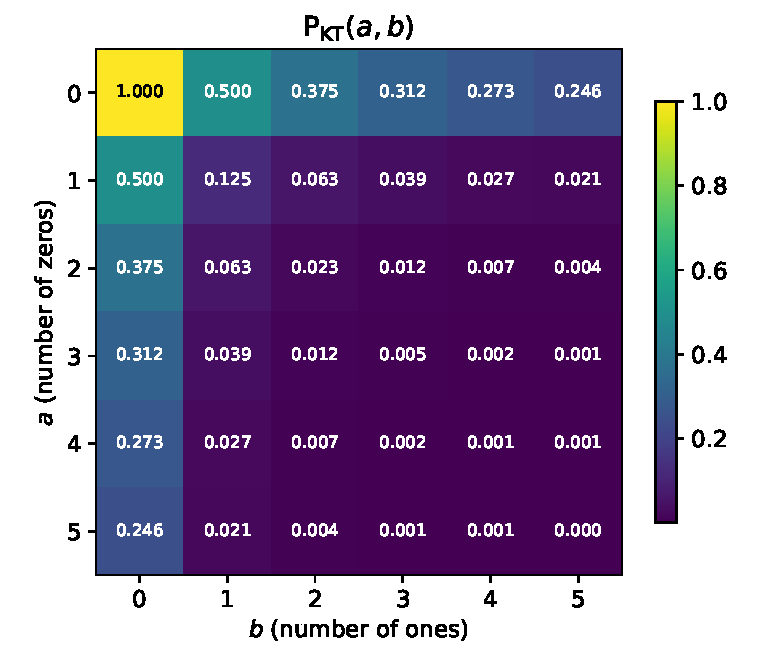
\includegraphics[width=0.48\linewidth]{py_kt_table}
\end{center}
\end{frame}

% ============================================================
\section{4.2 Context}

\begin{frame}{Why Context Matters}
The KT estimator only uses the \emph{frequency} of $\mathtt 0$s and $\mathtt 1$s; it
ignores the \emph{order} in which they appear. But for real sequences, recent history often
carries the most useful information --- this recent information is called the
\textbf{context}.

\begin{exampleblock}{Example 4.2.1 (Context in language)}
Given the letters \texttt{AD} and asked to guess the next letter of an English word, using
no context at all we would guess \texttt{E} (the most frequent letter overall) --- a poor
choice, since almost no words start with \texttt{ADE} or \texttt{ADT}. Conditioning on the
context \texttt{AD}, a good predictor assigns high probability to \texttt{V} and \texttt{J}
(words like \emph{advance}, \emph{adjust}), which the context-free frequency estimate would
never have suggested.
\end{exampleblock}
\end{frame}

\begin{frame}{Context Reshapes the Distribution}
\begin{center}
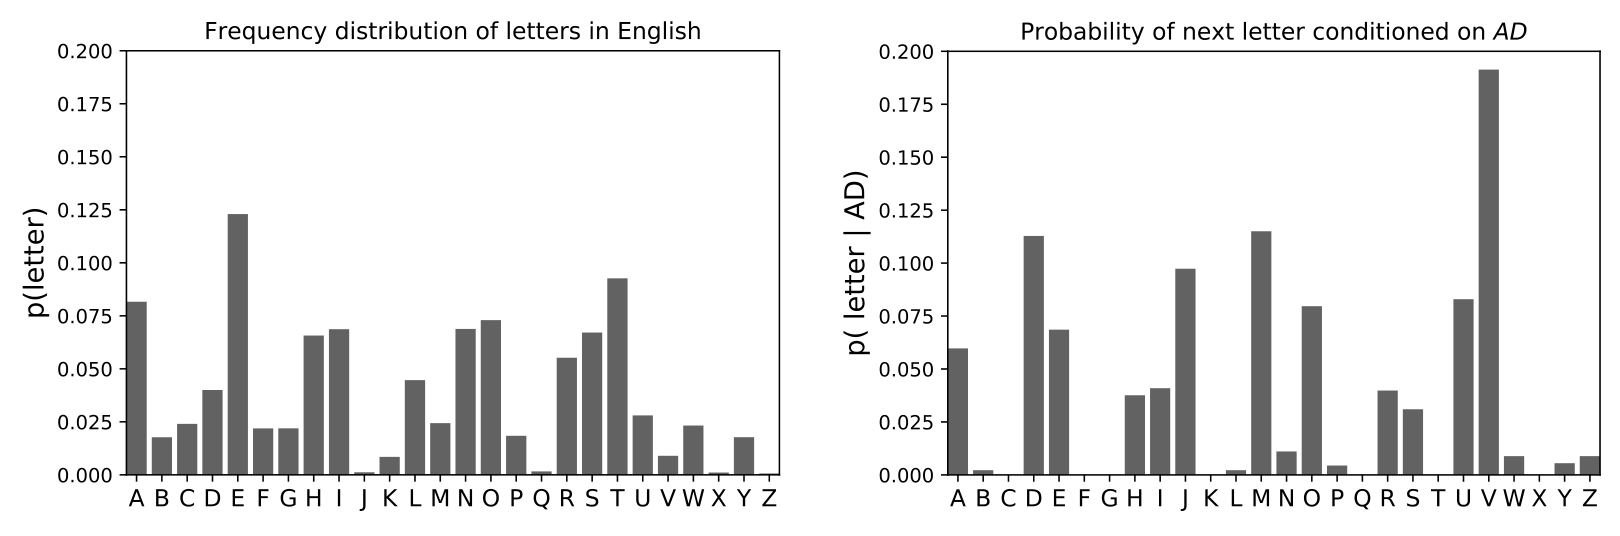
\includegraphics[width=0.92\linewidth]{fig4_2_3_letters}
\end{center}
Left: unconditional letter frequency in English. Right: probability of the next letter
given the context \texttt{AD} --- using context reshapes the distribution entirely.
\end{frame}

\begin{frame}{Markov Distributions}
\begin{block}{Definition 4.2.3 (Markov)}
A probability distribution $\mathrm{P}:\BB^*\to\Delta\BB$ is \emph{Markov} if
$\mathrm{P}(x_t\,|\,x_{<t}) = \mathrm{P}(x_t\,|\,x_{t-1})$ for all $t$: the distribution of
the next symbol depends \emph{only} on the single most recently observed symbol (and not on
the time step $t$ itself).
\end{block}
\textbf{Plain-English meaning:} once you know the very last bit, no earlier history helps
you predict the next bit any better. Every i.i.d.\ process is trivially Markov (it ignores
context entirely), so Markov is a strictly more general/powerful notion than i.i.d.

\begin{exampleblock}{Example 4.2.2 (KT fails on non-i.i.d.\ data)}
For the alternating sequence $x_{1:2t}=(\mathtt{01})^t$, the KT estimator gives
$\PKT(\mathtt 0\,|\,x_{1:2n})=\frac{n+\frac12}{2n+1}=\frac12$ — no better than a coin flip
— even though the pattern is perfectly predictable once you look at just the last bit.
\end{exampleblock}

\textbf{Remedy:} instead of counting single symbols, count \emph{digraphs} — how often each
symbol is followed by $\mathtt 0$ or $\mathtt 1$ — and run a separate KT estimator for each
possible ``most recent symbol.''
\end{frame}

\begin{frame}{$k$-Markov Environments}
\begin{block}{Definition 4.2.6 ($k$-Markov)}
$\mathrm{P}:\BB^*\to\Delta\BB$ is \emph{$k$-Markov} (a $k^{\mathrm{th}}$-order Markov
model) if $\mathrm{P}(x_t\,|\,x_{<t}) = \mathrm{P}(x_t\,|\,x_{t-k:t-1})$ for all $t$: the
next symbol depends only on the $k$ most recently observed symbols.
\end{block}
We define the \emph{KT counts} of a string $x$: $a_s(x)$ is the number of occurrences of
substring $s\mathtt 0$ in $x$, and $b_s(x)$ the number of occurrences of $s\mathtt 1$. Then
we run a KT estimator per context $s$:
$$
\mathrm{P}_k(\mathtt 0\,|\,x_{1:n}) = \frac{a_s+\tfrac12}{a_s+b_s+1}, \qquad
\mathrm{P}_k(\mathtt 1\,|\,x_{1:n}) = \frac{b_s+\tfrac12}{a_s+b_s+1} = 1-\mathrm{P}_k(\mathtt 0\,|\,x_{1:n})
$$
where $s = x_{n-k+1:n}$ is the most recent $k$ bits (\textbf{the context}).

\begin{exampleblock}{Example 4.2.5 (1-Markov KT)}
On the sequence $x_{1:6}=\mathtt{010101}$, since the most recent bit is $\mathtt 1$, we
count digraphs $\mathtt{10}$ (twice) and $\mathtt{11}$ (zero times), giving
$\mathrm{P}_1(x_7=\mathtt 0\,|\,x_{1:6})=\frac{2+\frac12}{2+0+1}=\frac56$: the 1-Markov
estimator is confidently correct, unlike the plain KT estimator.
\end{exampleblock}
\end{frame}

\begin{frame}{Choosing $k$: Too Small, Too Large}
\begin{exampleblock}{Example 4.2.8/2.9: $k=0,1,2$ on $(\mathtt{100})^n$}
On the sequence $(\mathtt{100})^n$ (a 2-Markov source), the $k$-Markov estimators give
$$
\mathrm{P}_0(\mathtt 0\,|\,(\mathtt{100})^n)\to\tfrac23,\qquad
\mathrm{P}_1(\mathtt 0\,|\,(\mathtt{100})^n)\to\tfrac12,\qquad
\mathrm{P}_2(\mathtt 0\,|\,(\mathtt{100})^n)\to 0.
$$
\end{exampleblock}
Only $k=2$ correctly learns the deterministic rule $\mathtt{00}\to\mathtt 1,\
\mathtt{01}\to\mathtt 0,\ \mathtt{10}\to\mathtt 0$. Surprisingly $k=1$ is \emph{worse} than
$k=0$: with only one bit of context, digraphs $\mathtt{01}$ and $\mathtt{00}$ occur about
equally often, so the 1-Markov model cannot tell them apart and gains nothing over the
naive (i.i.d.) estimate.

\begin{alertblock}{Remark 4.2.12 (Problem of $k$-Markov for large $k$)}
A $k$-Markov estimator has $2^k$ parameters to learn, so the sample size \emph{per
parameter} is only $O(n/2^k)$. Too small a $k$ means the model can never learn the true
pattern; too large a $k$ wastes data on irrelevant context and slows convergence. If the
environment truly is $k$-Markov but $k$ is unknown, we need a way to \emph{learn} the right
amount of context — this motivates variable-length context in Section 4.3.
\end{alertblock}
\end{frame}

\begin{frame}{$k$-Markov Experiments: A Noisy 2-Markov Source}
\begin{columns}
\begin{column}{0.45\textwidth}
Consider the 2-Markov chain $\mu_1$ below, parameterized by $\alpha$ (alpha)
$\in[0,1]$: with probability $\alpha$ the ``clean'' bit of the pattern $(\mathtt{100})^n$
is sampled, and with probability $1-\alpha$ a noisy/wrong bit is sampled instead (and the
context updates accordingly). Each state is labeled by its 2-bit context; edges show
(sampling probability, sampled bit).
\end{column}
\begin{column}{0.55\textwidth}
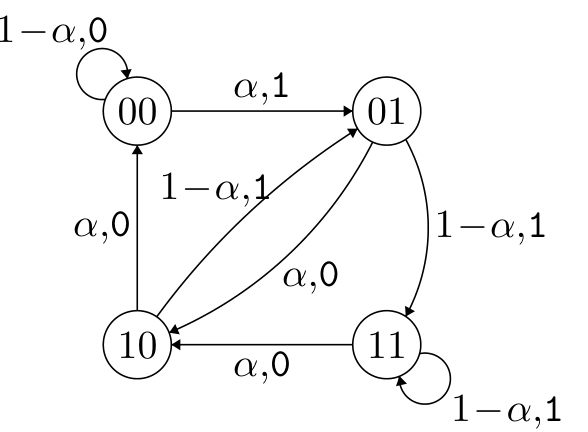
\includegraphics[width=\linewidth]{fig4_4_markov}
\end{column}
\end{columns}
\end{frame}

\begin{frame}{$k$-Markov Experiments: Accuracy and KL Divergence}
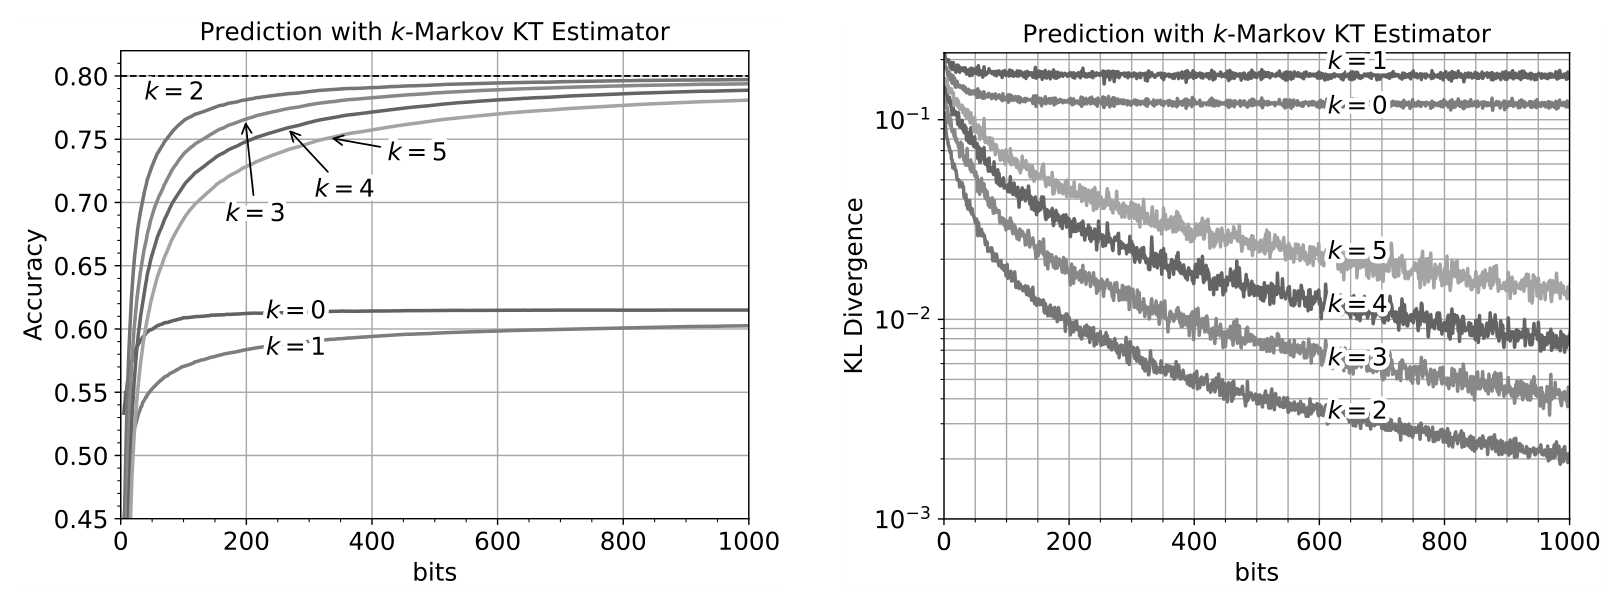
\includegraphics[width=0.95\linewidth]{fig4_5_kmarkov_exp}

Left: prediction accuracy vs. number of bits seen, for $k$-Markov KT
estimators, $\alpha=0.8$. Right: instantaneous KL divergence (Eq. 4.2.11) between the true
$\mu_1$ and each estimator's prediction --- lower is better. Any $k\ge2$ eventually learns the
pattern, but larger $k$ (more parameters) learns more slowly.
\end{frame}

\begin{frame}[fragile]{Python: $k$-Markov KT Estimator}
\begin{lstlisting}
def run_kmarkov_kt(bits, k):
    """Simulate a k-Markov KT estimator on a bit sequence, return per-step P(next=1)."""
    counts = {}   # context (tuple of k bits) -> [a, b]
    preds = []
    ctx = tuple([0] * k)  # pad with zeros before enough context accumulates
    for t, x in enumerate(bits):
        a, b = counts.get(ctx, [0, 0])
        p1 = (b + 0.5) / (a + b + 1)
        preds.append(p1)
        # update counts for the context we just used
        if x == 1:
            b += 1
        else:
            a += 1
        counts[ctx] = [a, b]
        # slide the context window forward by one bit
        ctx = (ctx + (x,))[-k:] if k > 0 else ()
    return preds

# demonstrate k=0 vs k=2 on (100)^n
bits = [1, 0, 0] * 40
p0 = run_kmarkov_kt(bits, k=0)
p2 = run_kmarkov_kt(bits, k=2)
print("k=0 final P(next=1):", round(p0[-1], 3))   # -> ~0.33 (matches global 1/3 frequency)
print("k=2 final P(next=1):", round(p2[-1], 3))   # -> ~0.0 or ~1.0 depending on context
\end{lstlisting}
\end{frame}

% ============================================================
\section{4.3 Variable Length Context}

\begin{frame}{Motivation: Not All Context Needs the Same Length}
A $k$-Markov estimator \emph{always} uses exactly $k$ bits of context, even when fewer
would do. Recall the optimal predictor for $\mu_1$ needs the rules
$\mathtt{00}\to\mathtt1,\ \mathtt{01}\to\mathtt0,\ \mathtt{10}\to\mathtt0,\ \mathtt{11}\to\mathtt0$
— but this simplifies to just
$$
\mathtt{00}\to\mathtt1 \qquad \mathtt{10}\to\mathtt0 \qquad \mathtt 1\to\mathtt0
$$
If the last bit was $\mathtt 1$, one bit of context suffices; only if the last bit was
$\mathtt 0$ do we need to look at the second-to-last bit too. We want predictors that can
use \emph{variable-length} context — long when needed, short when not.

\begin{exampleblock}{Example 4.3.1 (Context tree, in language)}
Given context \texttt{from the}, we may need to look further back (\texttt{run from the}
vs. \texttt{drink from the}) to decide \texttt{cop} vs. \texttt{cup}. But given context
\texttt{wash the}, no further context is needed — \texttt{cup} is almost certain. This
asymmetric context requirement is naturally represented as a tree:
\end{exampleblock}
\begin{center}
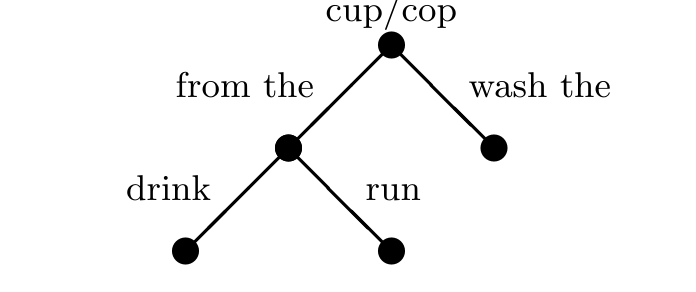
\includegraphics[width=0.45\linewidth]{fig4_6_context_tree}
\end{center}
\end{frame}

\begin{frame}{Suffixes and Suffix Sets}
\begin{block}{Definition 4.3.2 (Suffix)}
A string $x$ is a \emph{suffix} of string $y$ if there exists a string $z$ with $y=zx$.
\end{block}
E.g., $\mathtt{10}$ is a suffix of $\mathtt{0010}$.

\begin{block}{Definition 4.3.3 (Suffix set)}
A \emph{suffix set} $\mathcal{S}$ is a finite set of binary strings that is
\emph{complete} and \emph{proper}: it is \emph{proper} if no member of $\mathcal S$ is a
suffix of another member, and \emph{complete} if every semi-infinite (leftward) sequence
$\ldots x_{t-1}x_t$ has a suffix belonging to $\mathcal S$.
\end{block}
\textbf{Plain-English meaning:} a suffix set is a collection of ``recent-history patterns''
that (a) never overlap in a redundant way (properness) and (b) always has \emph{some}
pattern that matches any actual history (completeness) — so every possible context maps to
exactly one entry of $\mathcal S$.

\end{frame}

\begin{frame}{Uniqueness of Suffixes}
\begin{block}{Proposition 4.3.4 (Uniqueness of suffix)}
Given a suffix set $\mathcal S$, every semi-infinite sequence $\omega$ (omega) has a
\emph{unique} suffix in $\mathcal S$.
\end{block}

\begin{exampleblock}{Example 4.3.5}
$\mathcal S=\{\mathtt1,\mathtt{11},\mathtt{101},\mathtt{001}\}$ is proper and complete.
\end{exampleblock}
\end{frame}

\begin{frame}{Suffix Trees}
\begin{block}{Definition 4.3.6 (Suffix tree)}
A \emph{suffix tree} is a finite binary tree, defined recursively as
$$
\texttt{Tree = Leaf | Node Tree Tree}
$$
\end{block}
Every suffix set $\mathcal S$ corresponds to a unique suffix tree $\Psi_{\mathcal S}$: start
at a root node, and for each string $s\in\mathcal S$, read $s$ \textbf{in reverse (from
right to left)}, walking down the tree — a $\mathtt 0$ adds/walks to a \textbf{right} child,
a $\mathtt 1$ adds/walks to a \textbf{left} child. Reading in reverse reflects that the most
recent bit $x_n$ (the last one) should be examined \emph{first} when tracing context.

\begin{block}{Definition 4.3.7 (Model class $\mathcal{C}_D$)}
The model class of depth $D$ is the set of all complete, proper suffix sets with strings of
length at most $D$:
$$
\mathcal{C}_D := \begin{cases}
\{\{\epsilon\}\} & D=0\\
\{\{\epsilon\}\}\cup\{\mathcal S_1\{0\}\cup\mathcal S_2\{1\}:\mathcal S_1,\mathcal S_2\in\mathcal C_{D-1}\} & D>0
\end{cases}
$$
where $AB:=\{ab:a\in A,b\in B\}$ denotes concatenation of string sets.
\end{block}
\end{frame}

\begin{frame}{The Model Class $\mathcal C_D$: What It Means}
\textbf{Plain-English meaning:} $\mathcal C_D$ is simply the set of \emph{every} suffix set
that never needs more than $D$ bits of context — this is our model class, the collection of
all environments we are willing to consider.
\end{frame}

\begin{frame}{The Model Class $\mathcal{C}_D$ Grows Fast}
\begin{exampleblock}{Example 4.3.8}
$\mathcal C_0=\{\{\epsilon\}\}$, \quad
$\mathcal C_1 = \{\{\epsilon\},\{\mathtt0,\mathtt1\}\}$, \quad
$\mathcal C_2 = \{\{\epsilon\},\{\mathtt0,\mathtt1\},\{\mathtt{00},\mathtt{10},\mathtt1\},
\{\mathtt0,\mathtt{01},\mathtt{11}\},\{\mathtt{00},\mathtt{01},\mathtt{10},\mathtt{11}\}\}$
\end{exampleblock}

\begin{block}{Proposition 4.3.9 (Model class inclusions)}
$\mathcal C_0\subseteq \mathcal C_1\subseteq \mathcal C_2\subseteq \cdots$ — a deeper model
class contains every shallower one as a special case.
\end{block}

\begin{block}{Lemma 4.3.10 (Double-exponential size)}
For $D\ge1$: $\ 2^{2^{D-1}} \le |\mathcal C_D| \le 2^{2^D}$.
\end{block}
This is the key difficulty CTW must overcome: even $D=5$ gives a model class with roughly
$2^{32}\approx 4$ billion possible environments — far too many to enumerate one by one, yet
CTW will handle it in time \emph{linear} in $D$.

\begin{block}{Definition 4.3.11 (Prediction Suffix Tree, PST)}
A PST $\Psi_{\mathcal S,\Theta_{\mathcal S}}$ is a suffix tree whose leaves each carry a
parameter $\theta_s\in[0,1]$ (the probability the next bit is $\mathtt1$ given context $s$):
$\ \texttt{PST = Leaf}\ \theta\ \texttt{| Node PST PST}$.
\end{block}
\end{frame}

\begin{frame}{Predicting with a PST}
\begin{columns}
\begin{column}{0.42\textwidth}
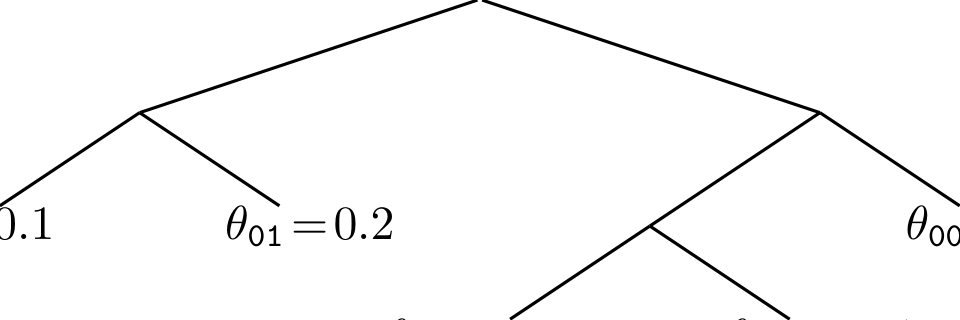
\includegraphics[width=\linewidth]{fig4_7_pst_tree}
\end{column}
\begin{column}{0.58\textwidth}
\begin{exampleblock}{Example 4.3.14}
For $\mathcal S=\{\mathtt{11},\mathtt{01},\mathtt{110},\mathtt{010},\mathtt{00}\}$ with
parameters $\theta_{11}{=}0.1,\theta_{01}{=}0.2,\theta_{110}{=}0.3,\theta_{010}{=}0.4,
\theta_{00}{=}0.5$: given the sequence $\mathtt{0101101}$, we compute $\beta_{\mathcal
S}(\mathtt{0101101})=\mathtt{01}$ (its suffix in $\mathcal S$), so
$$
\mathrm{P}_{\mathcal S,\Theta_{\mathcal S}}(x_t=1\,|\,x_{<t}=0101101) = \theta_{01} = 0.2.
$$
\end{exampleblock}
\end{column}
\end{columns}

\begin{block}{Definition 4.3.12 (Suffix function $\beta_{\mathcal S}$)}
$\beta_{\mathcal S}:\BB^\infty\to\BB^*$ maps a semi-infinite sequence onto its unique suffix
in $\mathcal S$. $\beta_{\mathcal S}$ depends only on the last $D:=\max_{s\in\mathcal
S}\ell(s)$ bits of the input (padding with zeros if fewer than $D$ bits are available).
\end{block}
\end{frame}

\begin{frame}{PST Probability as a Product}
\begin{block}{Lemma 4.3.16 (PST probability as a product)}
$$
\mathrm{P}_{\mathcal S,\Theta_{\mathcal S}}(x_{1:n}) = \prod_{s\in\mathcal S}\theta_s^{b_s}(1-\theta_s)^{a_s}
$$
where $a_s,b_s$ are the KT counts of $x_{1:n}$: the block probability factors into one term
per context in the suffix set, exactly as if we ran $|\mathcal S|$ independent i.i.d.\
processes.
\end{block}
\end{frame}

\begin{frame}{Algorithm 4.1: Building a PST from $(\mathcal S,\Theta_{\mathcal S})$}
\begin{block}{Algorithm 4.1 (Initializing PST from $\mathcal S$ and $\Theta_{\mathcal S}$)}
\begin{enumerate}
\item Initialize $\Psi$ as an empty binary tree.
\item For each $s\in\mathcal S$: set $p:=\Psi$ (start at root), and read $s$
\textbf{right-to-left}. For each bit: if it is $\mathtt1$, add/walk to the \textbf{left}
child of $p$; if it is $\mathtt 0$, add/walk to the \textbf{right} child.
\item Once $s$ is fully consumed, store $\theta_s$ in the current leaf node $p$.
\end{enumerate}
\end{block}
This is exactly how Figure 4.7's tree was built from
$\mathcal S=\{\mathtt{11},\mathtt{01},\mathtt{110},\mathtt{010},\mathtt{00}\}$.

\vspace{0.3cm}
\begin{block}{Encoding Suffix Sets: Definition 4.3.17 ($\mathcal E_D$)}
Given a fixed maximal depth $D$, a suffix tree $\Psi_{\mathcal S}$ is encoded as a bit
string: $\epsilon$ if $D=0$; $\mathtt 0$ if $\Psi_{\mathcal S}$ is a leaf; otherwise
$\mathtt1$ followed by the encodings of the left and right subtrees (at depth $D-1$).
Because the decoder knows the maximal depth $D$, this code is \emph{uniquely decodable}
(Theorem 4.3.19) even though some trees get surprisingly short codes.
\end{block}
\end{frame}

\begin{frame}{Encoding Examples for Depths $D=1,2,3$}
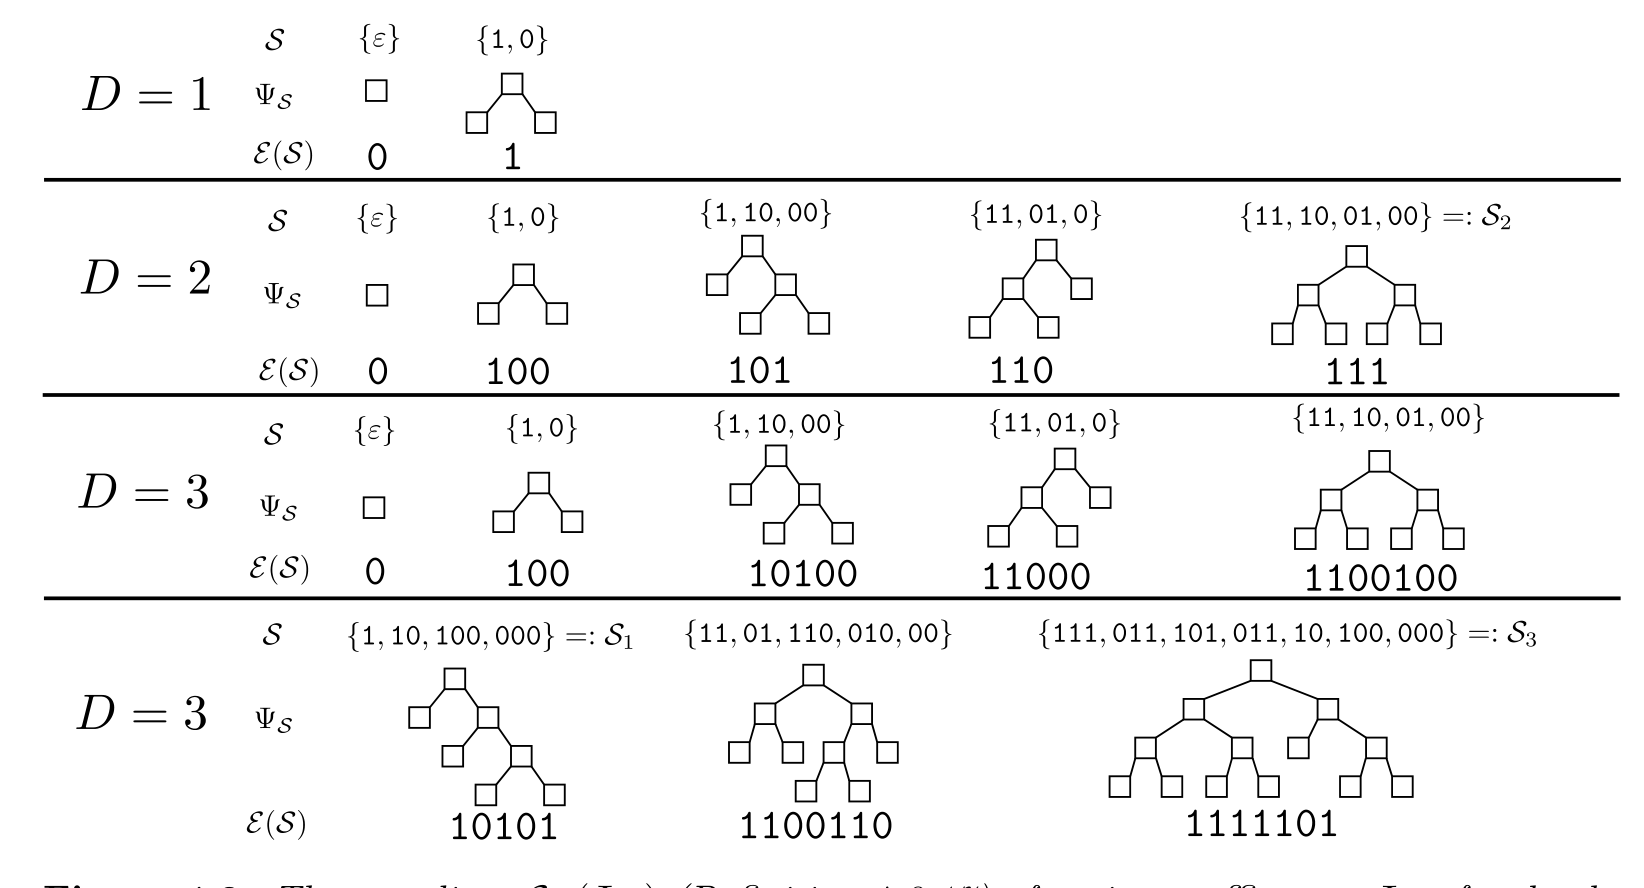
\includegraphics[width=0.95\linewidth]{fig4_8_encodings}
\end{frame}

\begin{frame}{Model Cost: How Complex is a Suffix Set?}
\begin{block}{Definition 4.3.20 (Model cost)}
$$
\Gamma_D(\mathcal S) := |\mathcal S| - 1 + |\{s\in\mathcal S:\ell(s)<D\}|
$$
\end{block}
\textbf{Plain-English meaning:} the model cost is the number of leaves in the suffix tree,
plus a penalty of $1$ for every leaf that is \emph{not} at the maximal depth $D$ (i.e. every
internal ``non-leaf'' node needs an extra bit to signal that it is not a leaf).

\begin{block}{Theorem 4.3.22 (Model cost = encoding length)}
$\Gamma_D(\mathcal S) = \ell(\mathcal E_D(\mathcal S))$: the model cost exactly equals the
number of bits used by the encoding $\mathcal E_D$.
\end{block}

\begin{exampleblock}{Example 4.3.23}
For $\mathcal S_1=\{\mathtt1,\mathtt{10},\mathtt{100},\mathtt{000}\}$ (deep, narrow tree)
and $\mathcal S_2=\{\mathtt{11},\mathtt{10},\mathtt{01},\mathtt{00}\}$ (shallow, balanced
tree), both with $4$ elements: $\Gamma_3(\mathcal S_1)=5$ but $\Gamma_2(\mathcal S_2)=3$.
\textbf{Balanced trees are cheaper} — the model cost rewards simplicity, which is exactly
what we want for a Bayesian prior that avoids overfitting to spurious deep context.
\end{exampleblock}
\end{frame}

\begin{frame}{Algorithms 4.2 \& 4.3: PST Prediction and Update}
\begin{block}{Algorithm 4.2 (Suffix Tree Prediction)}
\textbf{Input:} PST $\Psi_{\mathcal S,\Theta_{\mathcal S}}$, context $x_{1:t}$.\quad
\textbf{Output:} $\theta_{\beta_{\mathcal S}(x_{1:t})}$
\begin{enumerate}
\item For $i=t$ down to $1$: if $\Psi$ is a leaf, return $\Psi.\theta$; else walk to
$\Psi.\mathrm{left}$ if $x_i=\mathtt1$, else $\Psi.\mathrm{right}$.
\end{enumerate}
\end{block}

\begin{block}{Algorithm 4.3 (Suffix Tree Update)}
\textbf{Input:} PST updated on $x_{1:t}$; next bit $x=x_{t+1}$
\begin{enumerate}
\item Walk down the tree following $x_{1:t}$ (as in Algorithm 4.2) until reaching a leaf $s$.
\item If $x=\mathtt1$: $\Psi.b \mathrel{+}= 1$; else $\Psi.a\mathrel{+}=1$.
\item Update $\Psi.\theta := (\Psi.b+\tfrac12)/(\Psi.a+\Psi.b+1)$ — this is exactly the
recursive KT-estimator update (Lemma 4.1.2) applied at that one leaf.
\end{enumerate}
\end{block}
\textbf{PST-KT}: instead of fixing $\Theta_{\mathcal S}$ in advance, we \emph{learn} it
on-line using this update rule, giving the PST-KT probability
$\mathrm{P}_{\mathcal S,\mathrm{KT}}(x_{1:n}) = \prod_{s\in\mathcal S}\PKT(a_s,b_s)$
(Definition 4.3.24) — one independent KT estimator running at each leaf of the tree.
\end{frame}

\begin{frame}{PST Experiments: Known Structure Beats Fixed-$k$}
Comparing the PST predictor with known suffix set $\mathcal S_{\mathrm{good}}=\{\mathtt1,
\mathtt{10},\mathtt{00}\}$ (Figure 4.9, learned via Algorithm 4.3) against fixed $k$-Markov
KT estimators on the same noisy 2-Markov source $\mu_1$:

\begin{columns}
\begin{column}{0.4\textwidth}
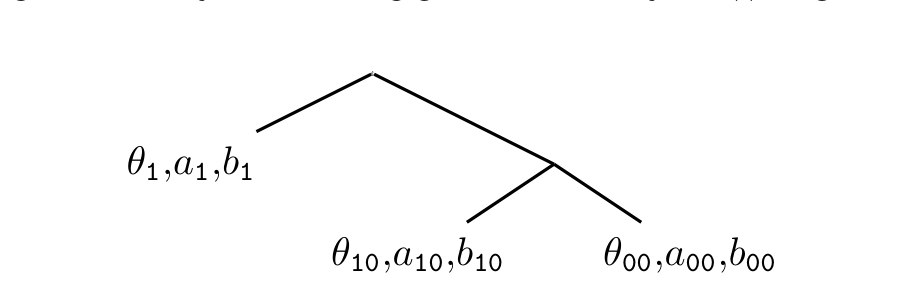
\includegraphics[width=\linewidth]{fig4_9_pst_good}
\end{column}
\begin{column}{0.6\textwidth}
Because $\mathcal S_{\mathrm{good}}$ already knows exactly which contexts matter (it merges
the redundant contexts $\mathtt{10}$ and $\mathtt{00}$ into the leaf $\mathtt1$), it has
fewer parameters to learn than $k=2$ or $k=3$, and hence learns \emph{faster} while being
just as accurate asymptotically.
\end{column}
\end{columns}
\vspace{0.2cm}
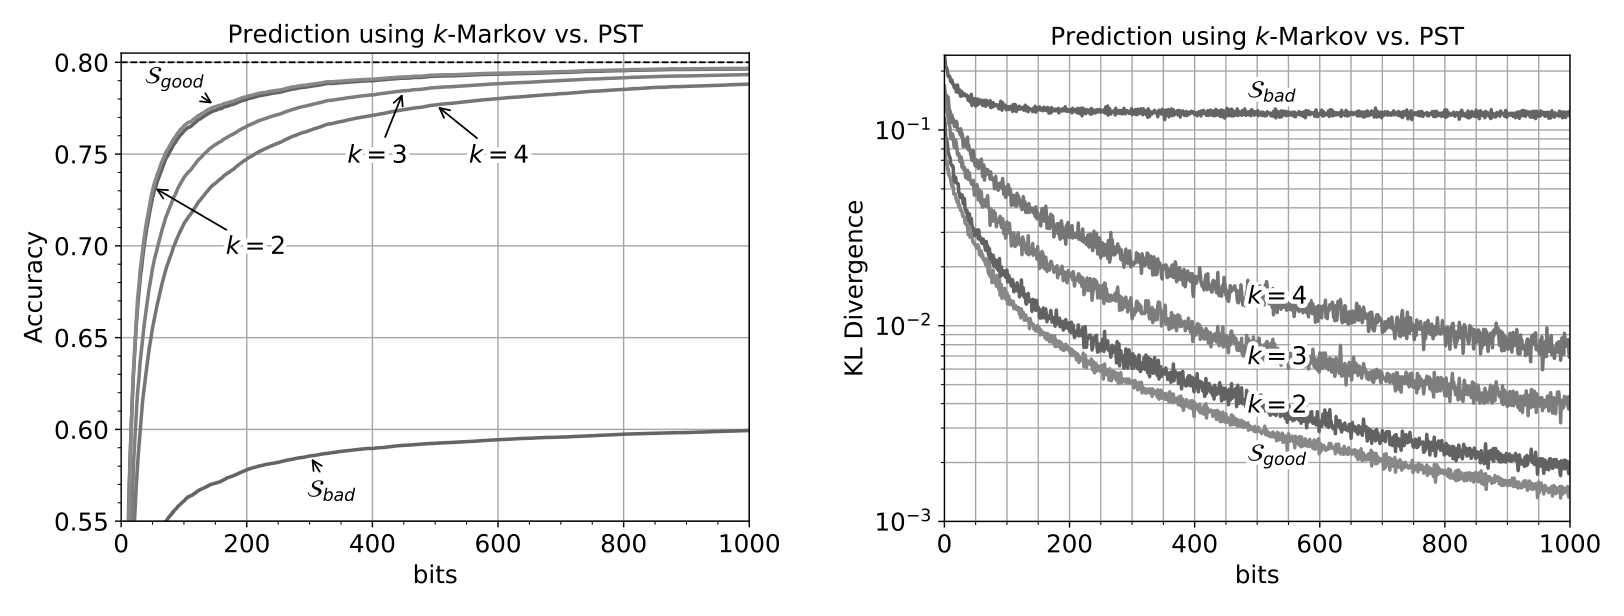
\includegraphics[width=0.9\linewidth]{fig4_10_pst_vs_k}

{\scriptsize $\mathcal S_{\mathrm{bad}}=\{\mathtt{11},\mathtt{01},\mathtt0\}$ (a
deliberately wrong suffix set) performs poorly throughout — choosing the wrong model
structure cannot be fixed just by learning parameters. This motivates \emph{learning the
structure too}, via a Bayesian mixture (Section 4.4).}
\end{frame}

% ============================================================
\section{4.4 Mixing Distributions}

\begin{frame}{Redundancy of Mixing Two Distributions}
\begin{exampleblock}{Example 4.4.1}
Suppose $\hat\mu_1$ predicts $\mu_1$ well and $\hat\mu_2$ predicts $\mu_2$ well. Consider
the simple average mixture $\hat\mu_w(x_{1:t}):=\tfrac12\hat\mu_1(x_{1:t})+\tfrac12\hat\mu_2(x_{1:t})$.
Then for either $i\in\{1,2\}$:
$$
r_{\hat\mu_w,\mu_i}(x_{1:n}) = \log_2\frac{2}{\hat\mu_1(x_{1:t})+\hat\mu_2(x_{1:t})} -
\log_2\frac{1}{\mu_i(x_{1:t})} \le 1 + r_{\hat\mu_i,\mu_i}.
$$
\end{exampleblock}
\textbf{Plain-English meaning:} mixing two good predictors together costs at most \emph{one
extra bit} of redundancy compared to using the best one alone — yet we get a single
predictor that works well \emph{no matter which} of the two environments is the true one.
This is the core insight behind Bayesian mixtures: hedging your bets across many models is
nearly free if you already have a good model for each possibility, and the same argument
extends to an uneven mixture $\hat\mu_{w,\alpha}=\alpha\hat\mu_1+(1-\alpha)\hat\mu_2$, or a
mixture of arbitrarily many distributions with weights $\theta_i\ge0,\sum_i\theta_i=1$.

\vspace{0.2cm}
Since $\mathcal C_D$ can have up to $2^{2^D}$ suffix sets, we cannot afford one extra bit
\emph{per suffix set} in a naive mixture — we need a way to mix over \emph{all} of
$\mathcal C_D$ at once, efficiently. That is exactly what CTW does.
\end{frame}

% ============================================================
\section{4.5 Context Tree Weighting}

\begin{frame}{Setup}
We now assume only that the true environment $\mu$ is \emph{some} $\mathrm{P}_{\mathcal
S,\Theta_{\mathcal S}}$ for an \emph{unknown} suffix set $\mathcal S$ and unknown parameters
$\Theta_{\mathcal S}$, with the (weak) assumption that we know an upper bound $D$ on how
much context could ever be needed (so $\mathcal S\in\mathcal C_D$).

The natural Bayesian approach: fix the model class $\mathcal C_D$, put a prior weight
$w_{\mathcal S}$ on each suffix set, and use the Bayes mixture (recall Section 3.1):
$$
\xi(x_{1:n}) := \sum_{\mathcal S\in\mathcal C_D} w_{\mathcal S}\,\mathrm{P}_{\mathcal
S,\Theta_{\mathcal S}}(x_{1:n})
$$
Naively this costs $O(2^{2^D})$ time — utterly infeasible even for modest $D$. \textbf{CTW}
computes exactly this mixture (with weights $w_{\mathcal S}:=2^{-\Gamma_D(\mathcal S)}$) in
only $O(n\cdot D)$ time.
\end{frame}

\begin{frame}[allowframebreaks]{4.5.1 The CTW Algorithm}
\begin{block}{Definition 4.5.1 (Context tree)}
Given depth $D$, a \emph{context tree} $\mathcal T_D$ is a \emph{perfect} binary tree where
every node $s$ (path of length $\ell(s)\le D$ from the root) stores KT counts $(a_s,b_s)$,
the KT probability $\PKT(a_s,b_s)$, and a \emph{weighted probability} $\Pw(s)$ defined
recursively:
$$
\Pw(s) := \begin{cases}
\tfrac12\PKT(a_s,b_s) + \tfrac12\Pw(\mathtt0 s)\Pw(\mathtt1 s) & \ell(s)<D\\
\PKT(a_s,b_s) & \ell(s)=D
\end{cases}
$$
where $\mathtt1 s$ and $\mathtt0 s$ are the left/right children (context with a $\mathtt1$
or $\mathtt0$ prepended), and $a_s=a_{\mathtt1 s}+a_{\mathtt0 s}$,
$b_s=b_{\mathtt1 s}+b_{\mathtt0 s}$.
\end{block}
\textbf{Plain-English meaning:} at every leaf ($\ell(s)=D$), we simply run the ordinary KT
estimator, exactly as if the sequence following context $s$ were i.i.d. At every internal
node, we \emph{mix} two hypotheses with equal weight $\tfrac12$ each: either the KT
estimator here is already good enough (first term), or we should look one bit deeper into
the context and combine the (already-computed) weighted probabilities of both children
(second term). This mirrors exactly the redundancy argument from Example 4.4.1.

\framebreak

\begin{block}{Algorithm 4.4 (CTW Update, conceptual)}
For each new bit $x_{t+1}$, using its $D$-bit context $x_{t-D+1:t}$:
\begin{enumerate}
\item Walk from the root to the leaf $s$ that matches the context, and at every node $s'$
along the way update $a_{s'},b_{s'}$ and $\PKT(a_{s'},b_{s'})$ (Lemma 4.1.2).
\item Walk back up from the leaf to the root, and at each node recompute
$\Pw(s')=\tfrac12\PKT(a_{s'},b_{s'})+\tfrac12\Pw(\mathtt0 s')\Pw(\mathtt1 s')$.
\end{enumerate}
\end{block}
Each update touches only the $D$ nodes on the path from root to leaf, so the whole update
costs $O(D)$ time — regardless of how large $\mathcal C_D$ is!

\begin{block}{Definition 4.5.4 (CTW probability)}
$\mathrm{P}_D^{\mathrm{CTW}}(x_{1:n}) := \Pw(\epsilon)$, the weighted probability at the
root after processing $x_{1:n}$. The conditional (predictive) probability is recovered as
$$
\mathrm{P}_D^{\mathrm{CTW}}(1\,|\,x_{<n}) = \frac{\mathrm{P}_D^{\mathrm{CTW}}(x_{<n}1)}{\mathrm{P}_D^{\mathrm{CTW}}(x_{<n})}.
$$
\end{block}

\framebreak

\begin{exampleblock}{Example 4.5.6 (Walking through a $D=2$ update)}
Start with a freshly initialized tree $\mathcal T_2$ (all counts zero, all
$\PKT=\Pw=1$):
\end{exampleblock}
\begin{center}
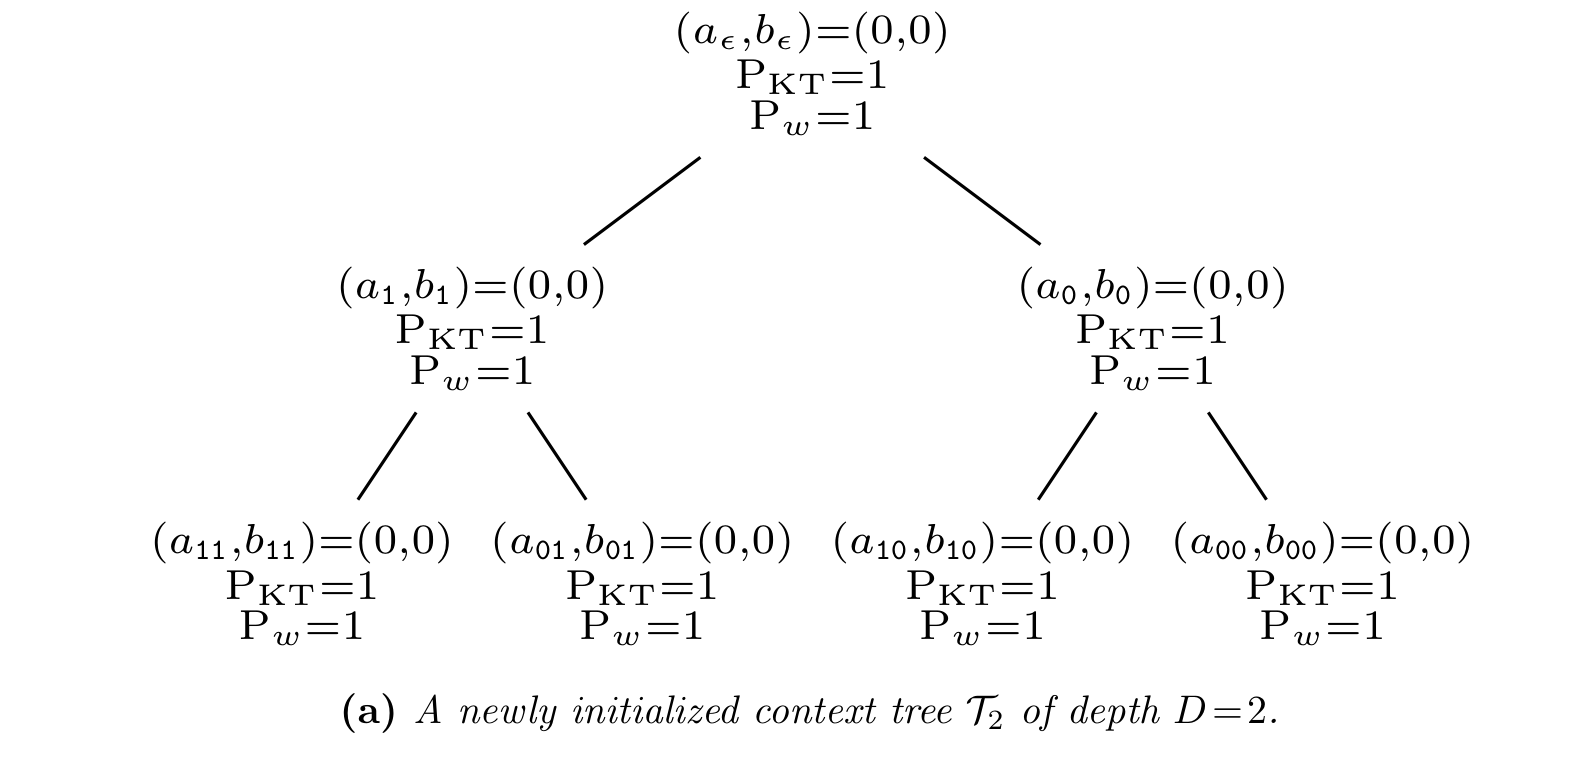
\includegraphics[width=0.62\linewidth]{fig4_11a_ctw_init}
\end{center}

\framebreak

Feed in $x_{1:4}=\mathtt{1001}$. After observing $x_3=\mathtt0$ given context $x_{1:2}=\mathtt{10}$
(the path $\epsilon\to\mathtt0\to\mathtt{10}$ is updated, highlighted in black):
\begin{center}
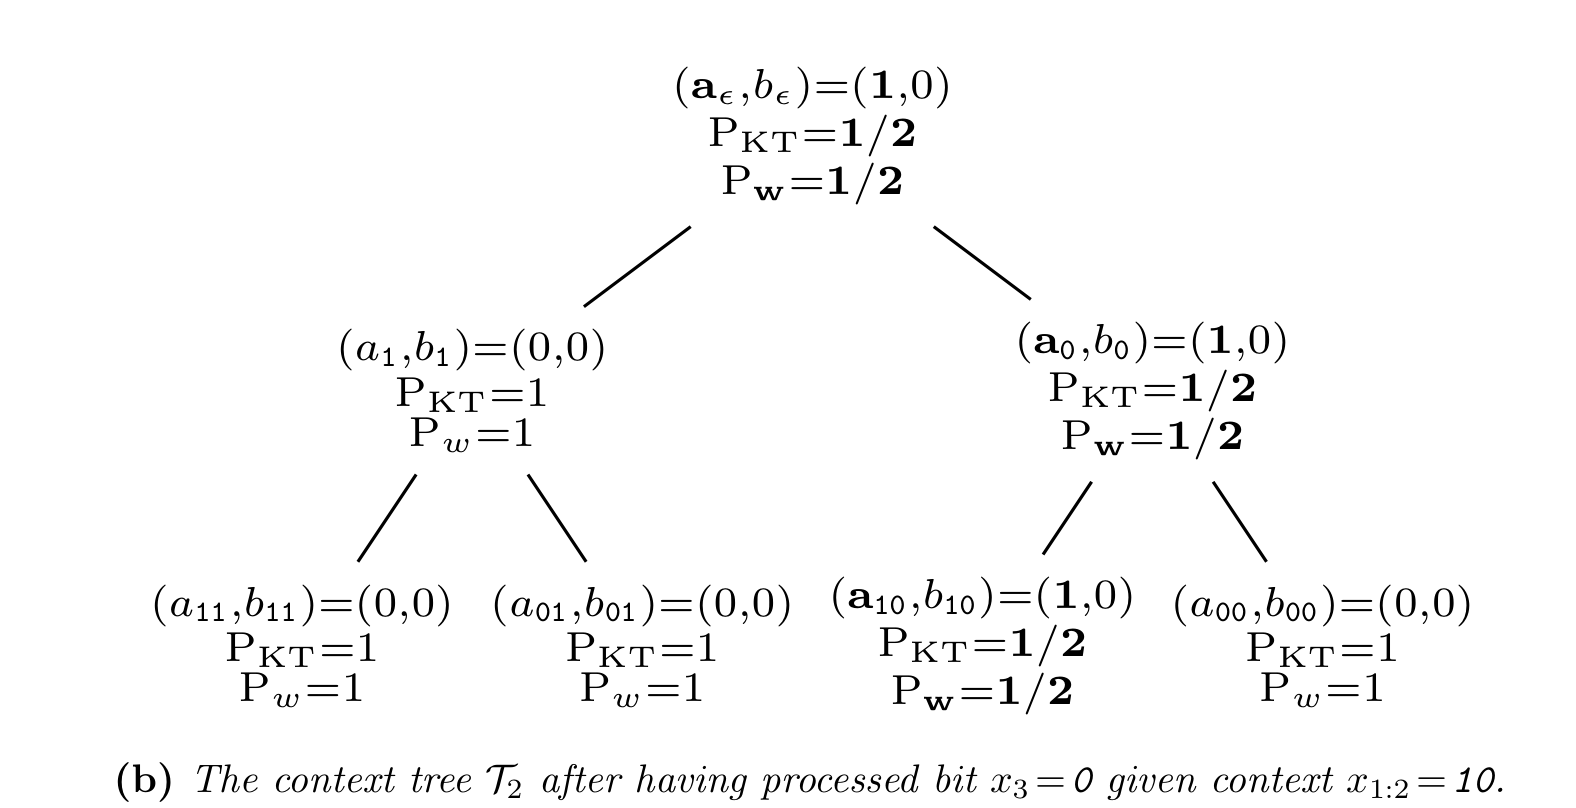
\includegraphics[width=0.62\linewidth]{fig4_11b_ctw_step1}
\end{center}

\framebreak

Then after observing $x_4=\mathtt1$ given context $x_{1:3}=\mathtt{100}$ (path
$\epsilon\to\mathtt0\to\mathtt{00}$ updated):
\begin{center}
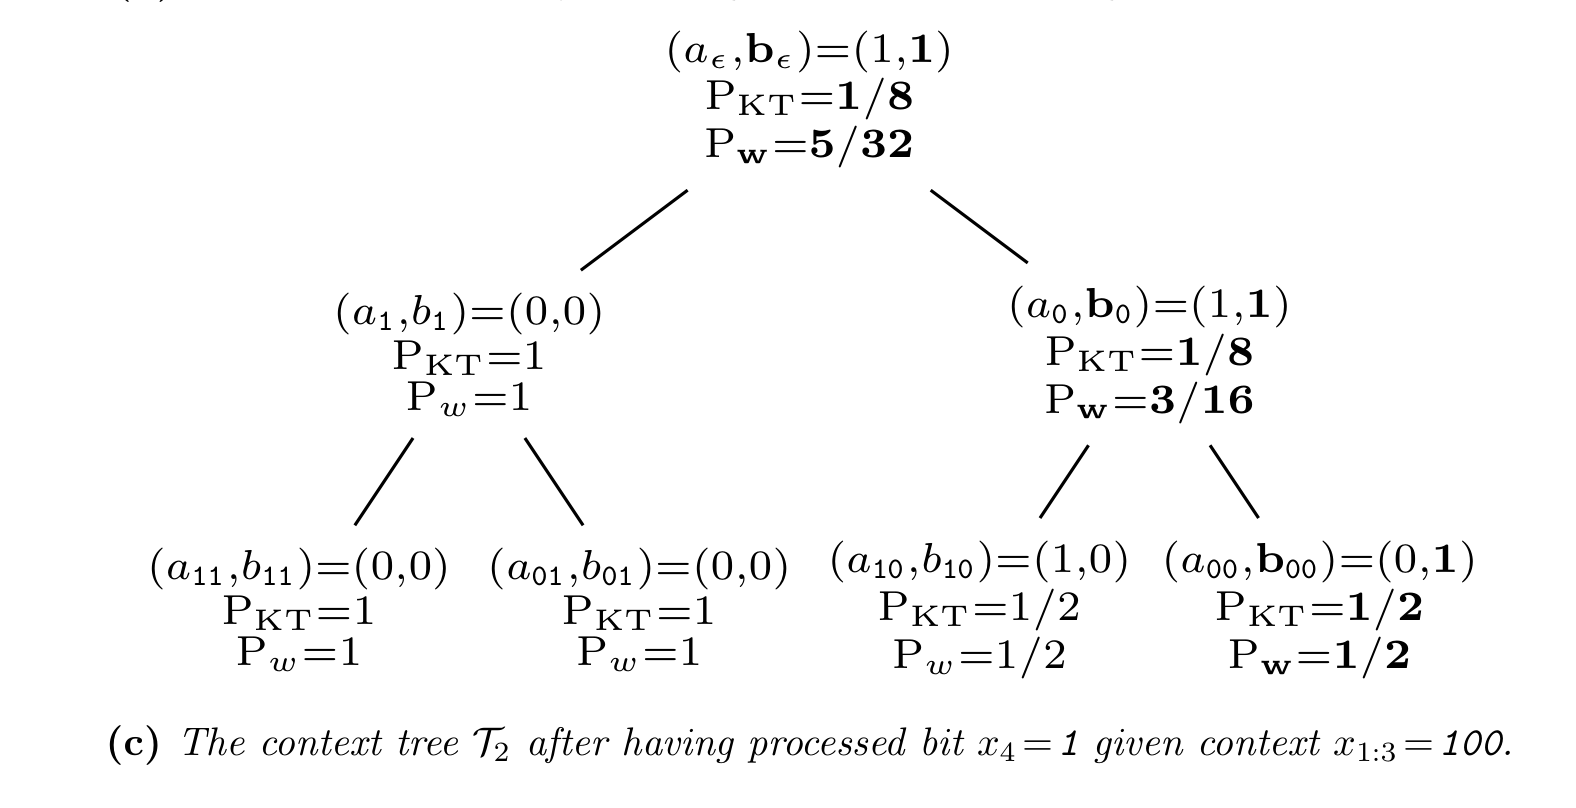
\includegraphics[width=0.62\linewidth]{fig4_11c_ctw_step2}
\end{center}
Notice how $\Pw(\epsilon)=5/32$ at the root combines information from \emph{both} updates —
this single number already represents the Bayes mixture over \emph{all five} suffix sets in
$\mathcal C_2$ (Remark 4.5.7).
\end{frame}

\begin{frame}{Unrolling $\Pw(\epsilon)$ for Small $D$}
\begin{block}{Remark 4.5.7 (CTW is a mixture over all PSTs)}
For $D=0$: $\Pw(\epsilon)=\PKT(a,b)$ (plain KT). For $D=1$, writing $k(s):=\PKT(a_s,b_s)$:
$$
\Pw(\epsilon) = \tfrac12 k(\epsilon) + \tfrac12 k(\mathtt0)k(\mathtt1)
$$
For $D=2$, expanding fully:
$$
\Pw(\epsilon) = \tfrac12\,\square + \tfrac18\Big(\wedge + {\scriptstyle\hat{\ }}\!\wedge +
\wedge\!{\scriptstyle\hat{\ }} + \wedge\wedge\Big)
$$
where each symbol corresponds to one of the five trees in $\mathcal C_2$: the empty tree
$\square$ gets weight $2^{-1}$ (model cost $1$), and each of the other four (depth-2) trees
gets weight $2^{-3}$ (model cost $3$) — matching Figure 4.8's encoding lengths exactly!
\end{block}
\begin{center}
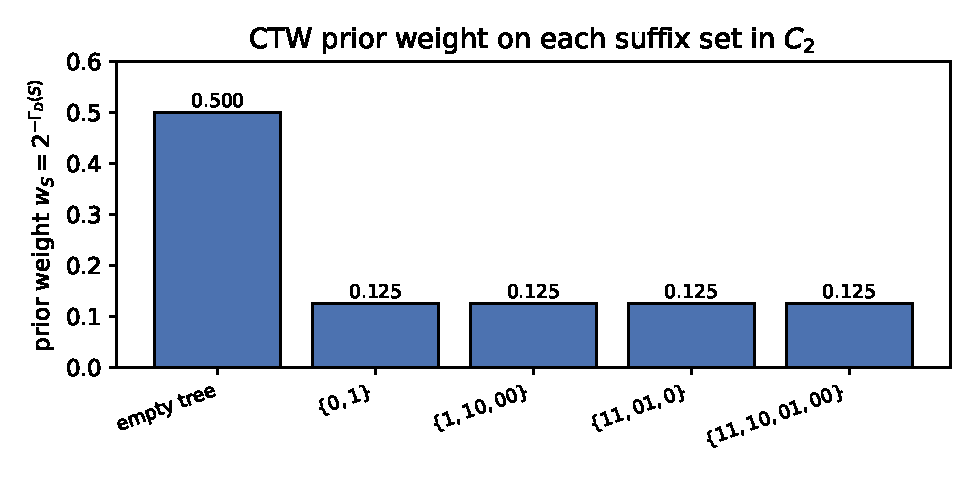
\includegraphics[width=0.75\linewidth]{py_ctw_prior_weights}
\end{center}
\end{frame}

\begin{frame}{4.5.2 CTW Properties: The Main Theorem}
\begin{block}{Theorem 4.5.8 (Context Tree Weighting)}
For any node $s\in\mathcal T_D$ with $d=\ell(s)$, and counts taken w.r.t.\ $x_{1:n}$:
$$
\Pw(s) = \sum_{\mathcal S\in\mathcal C_{D-d}} 2^{-\Gamma_{D-d}(\mathcal S)}
\prod_{s'\in\mathcal S}\PKT(a_{s's},b_{s's})
$$
\end{block}
\textbf{Proof idea:} by reverse induction on depth, using the recursive model-cost identity
$\Gamma_{D+1}(\mathcal V\{0\}\cup\mathcal W\{1\})=\Gamma_D(\mathcal V)+\Gamma_D(\mathcal W)+1$
(Lemma 4.3.21) to show that splitting $\Pw(s)$ into its KT term and its two-children term is
exactly equivalent to summing over all ways of extending a suffix set one level deeper.
\end{frame}

\begin{frame}{The Headline Result: CTW is an Exact Bayes Mixture}
\begin{block}{Theorem 4.5.11 (Bayesian mixture over suffix sets)}
$$
\mathrm{P}_D^{\mathrm{CTW}}(x_{1:n}) = \sum_{\mathcal S\in\mathcal C_D} w_{\mathcal S}\,
\mathrm{P}_{\mathcal S,\mathrm{KT}}(x_{1:n}), \qquad w_{\mathcal S}:=2^{-\Gamma_D(\mathcal S)}
$$
\end{block}
\textbf{This is the headline result:} the CTW root value \emph{is exactly} the Bayes mixture
we wanted from Section 4.5, computed in $O(nD)$ time instead of the naive $O(2^{2^D})$ — a
double-exponential speedup, and the weights $w_{\mathcal S}=2^{-\Gamma_D(\mathcal S)}$ form a
valid probability distribution over $\mathcal C_D$ (Lemma 4.5.10) that favors simpler
(more balanced, shallower) suffix sets, exactly as a good Occam's-razor-style prior should.
\end{frame}

\begin{frame}{4.5.3 CTW--PST--KT Redundancy Chain}
Convergence properties propagate up the chain KT $\to$ PST-KT $\to$ CTW:

\begin{block}{Theorem 4.5.12 (PST-KT redundancy)}
For any $\mathcal S\in\mathcal C_D$ and parameters $\Theta_{\mathcal S}$,
$$
\log_2\mathrm{P}_{\mathcal S,\Theta_{\mathcal S}}(x_{1:n}) - \log_2\mathrm{P}_{\mathcal
S,\mathrm{KT}}(x_{1:n}) \le |\mathcal S|\,\gamma(n/|\mathcal S|), \qquad
\gamma(t):=\tfrac12\log_2(t)+1 \text{ for } t\ge1.
$$
\end{block}

\begin{block}{Lemma 4.5.13 (CTW-KT redundancy)}
$\log_2\mathrm{P}_{\mathcal S,\mathrm{KT}}(x_{1:n}) - \log_2\mathrm{P}_D^{\mathrm{CTW}}(x_{1:n})
\le \Gamma_D(\mathcal S)$.
\end{block}

\begin{block}{Corollary 4.5.14 (PST-CTW redundancy, combined)}
$$
\log_2\mathrm{P}_{\mathcal S,\Theta_{\mathcal S}}(x_{1:n}) - \log_2\mathrm{P}_D^{\mathrm{CTW}}(x_{1:n})
\le \tfrac12|\mathcal S|\log_2 n + \Gamma_D(\mathcal S) + |\mathcal S|
$$
\end{block}
\textbf{Plain-English meaning:} the total extra cost of using CTW instead of knowing the
exact true model in advance grows only like $\tfrac12\log_2 n$ per parameter — this matches
the \emph{Rissanen lower bound}, the best possible redundancy for \emph{any} estimator, so
CTW is asymptotically optimal.
\end{frame}

\begin{frame}{4.5.4 CTW Experiments}
Comparing CTW (depths $D=2,3$) against the PST with known $\mathcal S_{\mathrm{good}}$ and
the $2$-Markov KT estimator, all on the same environment $\mu_1$:
\begin{center}
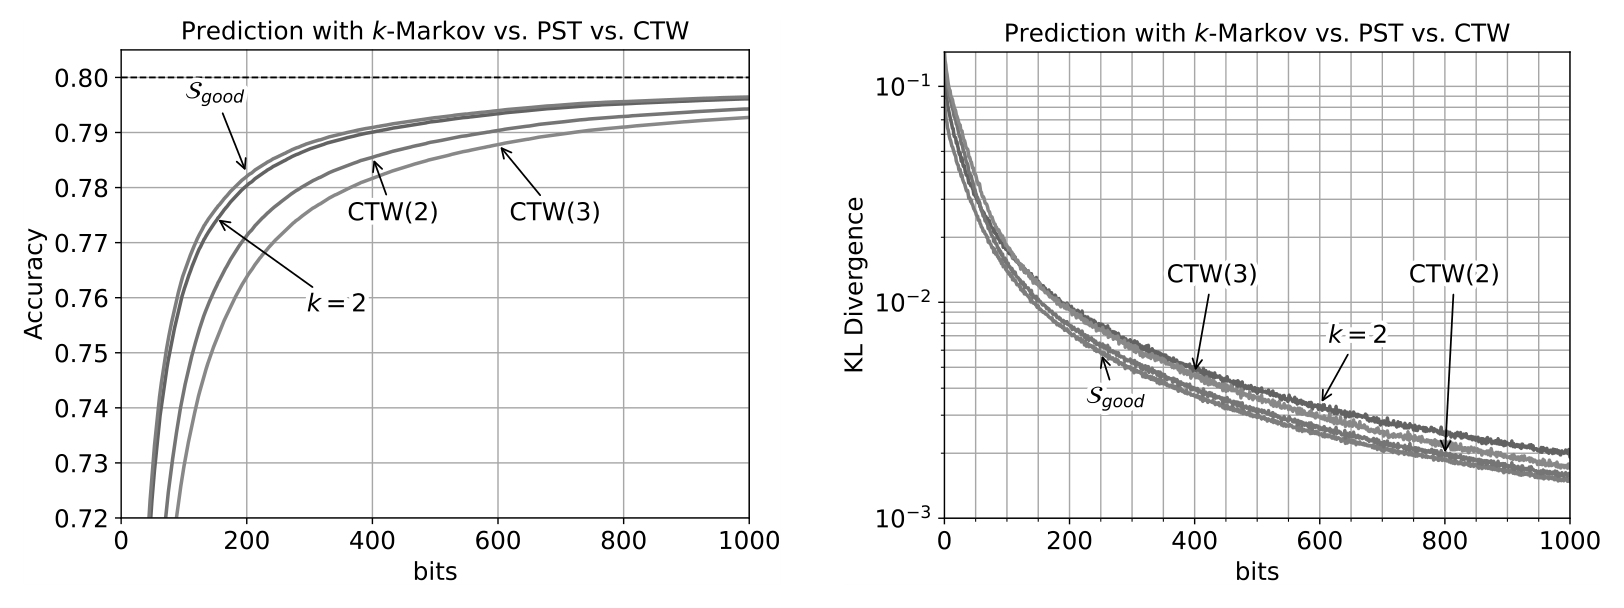
\includegraphics[width=0.92\linewidth]{fig4_12_ctw_exp}
\end{center}
\end{frame}

\begin{frame}{CTW Experiments: Discussion}
\begin{itemize}
\item The PST with known structure is best (it never has to \emph{learn} which contexts
matter).
\item CTW($D{=}2$) is close behind, since $D=2$ already contains $\mathcal S_{\mathrm{good}}$
in its model class and quickly concentrates its mixture weight there.
\item CTW($D{=}3$) is slightly slower, since its larger model class
($\mathcal C_3\supset\mathcal C_2$) spreads the prior more thinly, giving
$\mathcal S_{\mathrm{good}}$ a smaller a-priori weight.
\item The plain 2-Markov KT estimator is worst --- it can never discover the
variable-length structure at all, no matter how much data it sees.
\end{itemize}
\end{frame}

\begin{frame}[fragile]{Python: A Minimal CTW Implementation (I)}
\begin{lstlisting}
class CTWNode:
    def __init__(self):
        self.a = self.b = 0
        self.P_kt = 1.0
        self.P_w = 1.0
        self.children = [None, None]   # [right (bit=0), left (bit=1)]

class CTW:
    def __init__(self, depth):
        self.D = depth
        self.root = CTWNode()

    def _get_or_make(self, node, bit):
        if node.children[bit] is None:
            node.children[bit] = CTWNode()
        return node.children[bit]
\end{lstlisting}
Each \texttt{CTWNode} stores exactly the four quantities from Definition 4.5.1: the KT
counts $(a,b)$, the KT probability $\PKT(a,b)$, and the weighted probability $\Pw$. Nodes
are created lazily by \texttt{\_get\_or\_make} --- this is the online-initialization
optimization from Section 4.5.5.
\end{frame}

\begin{frame}[fragile]{Python: A Minimal CTW Implementation (II)}
\begin{lstlisting}
    def update(self, context_bits, x):
        """context_bits: most-recent-first list of the D bits preceding x."""
        path = [self.root]
        node = self.root
        for i in range(self.D):
            node = self._get_or_make(node, context_bits[i])
            path.append(node)
        for node in path:                                  # update KT stats
            if x == 1:
                node.P_kt *= (node.b + 0.5) / (node.a + node.b + 1); node.b += 1
            else:
                node.P_kt *= (node.a + 0.5) / (node.a + node.b + 1); node.a += 1
        leaf = path[-1]
        leaf.P_w = leaf.P_kt
        for node in reversed(path[:-1]):                   # recompute P_w bottom-up
            left = node.children[1].P_w if node.children[1] else 1.0
            right = node.children[0].P_w if node.children[0] else 1.0
            node.P_w = 0.5 * node.P_kt + 0.5 * left * right

# reproduce Example 4.5.6 on D=2, sequence 1001
ctw = CTW(depth=2)
ctx = [0, 0]                       # pad with zeros: no history yet
for x in [1, 0, 0, 1]:
    ctw.update(ctx, x)
    ctx = [x] + ctx[:1]            # most-recent-first context of length D=2
    print("P_w(root) =", ctw.root.P_w)
# Final output matches P_w(epsilon) = 5/32 = 0.15625 from Figure 4.11(c)
\end{lstlisting}
\end{frame}

\begin{frame}[allowframebreaks]{4.5.5 Optimizations}
\textbf{1. Log probabilities.} Since $\mathrm{P}_{\mathcal S,\mathrm{KT}}(x_{1:n})$ shrinks
exponentially in $n$, ordinary 64-bit floats underflow after only a few hundred bits. The
fix: store $\log_2\PKT$ and $\log_2\Pw$ instead, using the numerically stable log-sum
operator
$$
a\oplus b := \max\{a,b\} + \log_2\!\left(1+2^{\min\{a,b\}-\max\{a,b\}}\right)
$$
which computes $\log_2(2^a+2^b)$ without ever exponentiating a very negative number. The
update rule (4.5.2) becomes
$$
\log_2\Pw(s) = \big[\log_2\PKT(a_s,b_s)\ \oplus\ (\log_2\Pw(\mathtt0 s)+\log_2\Pw(\mathtt1 s))\big] - 1
\quad\text{for } \ell(s)<D.
$$

\framebreak

\textbf{2. Online (lazy) tree initialization.} The full context tree $\mathcal T_D$ has
$O(2^D)$ nodes, intractable to allocate up front for even moderate $D$. Instead:
\begin{itemize}
\item Start with just the root node. Treat all other nodes as \texttt{null} (unallocated,
implicitly $(a,b)=(0,0)$, $\PKT=1$, $\Pw=1$).
\item Only ever create a node the first time its context is actually observed (Algorithm
4.6). Since $\Pw=1$ for every null node regardless of depth, formula (4.5.2) simplifies:
$$
\Pw(s) = \begin{cases} 1 & s \text{ is null} \\ \tfrac12\PKT(a_s,b_s)+\tfrac12\Pw(\mathtt0
s)\Pw(\mathtt1 s) & \ell(s)<D,\ s\text{ allocated} \\ \PKT(a_s,b_s) & \ell(s)=D \end{cases}
$$
\end{itemize}
This bounds the number of allocated nodes by $O(nD)$ — in practice far fewer, since many
contexts are never seen.
\begin{center}
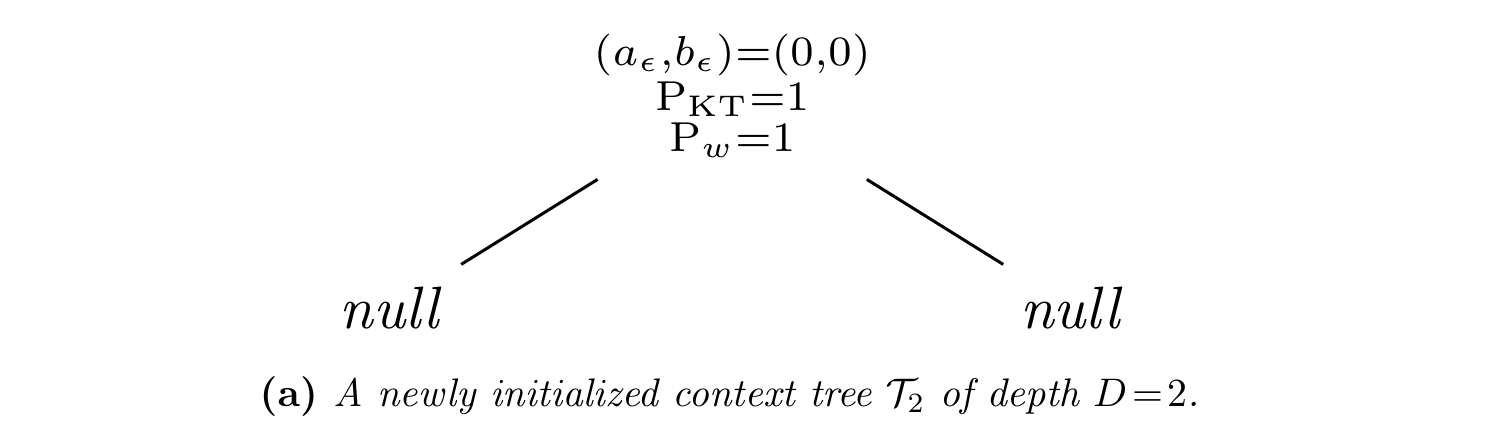
\includegraphics[width=0.6\linewidth]{fig4_13a_online_init}
\end{center}

\framebreak

\begin{columns}
\begin{column}{0.5\textwidth}
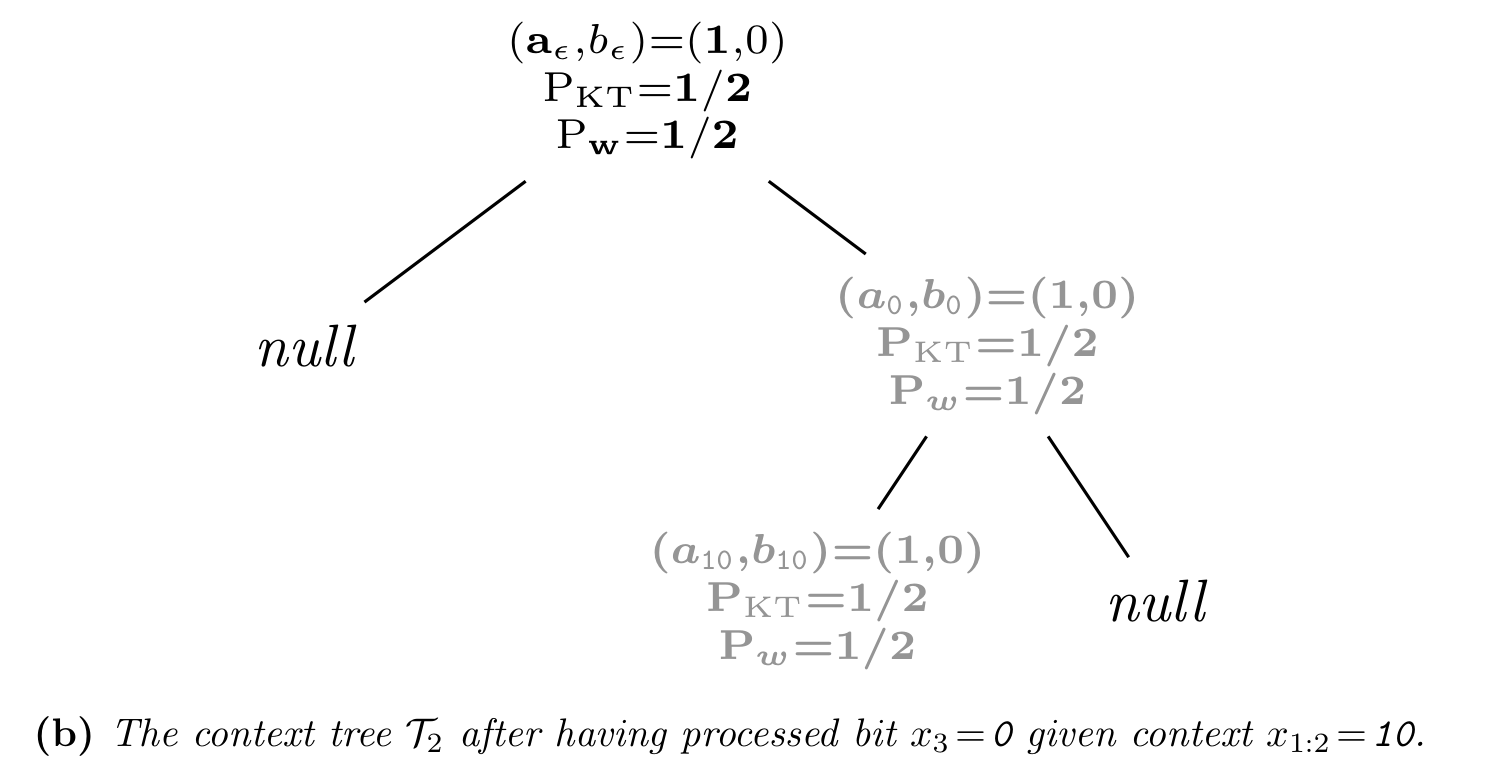
\includegraphics[width=\linewidth]{fig4_13b_online_step1}
\end{column}
\begin{column}{0.5\textwidth}
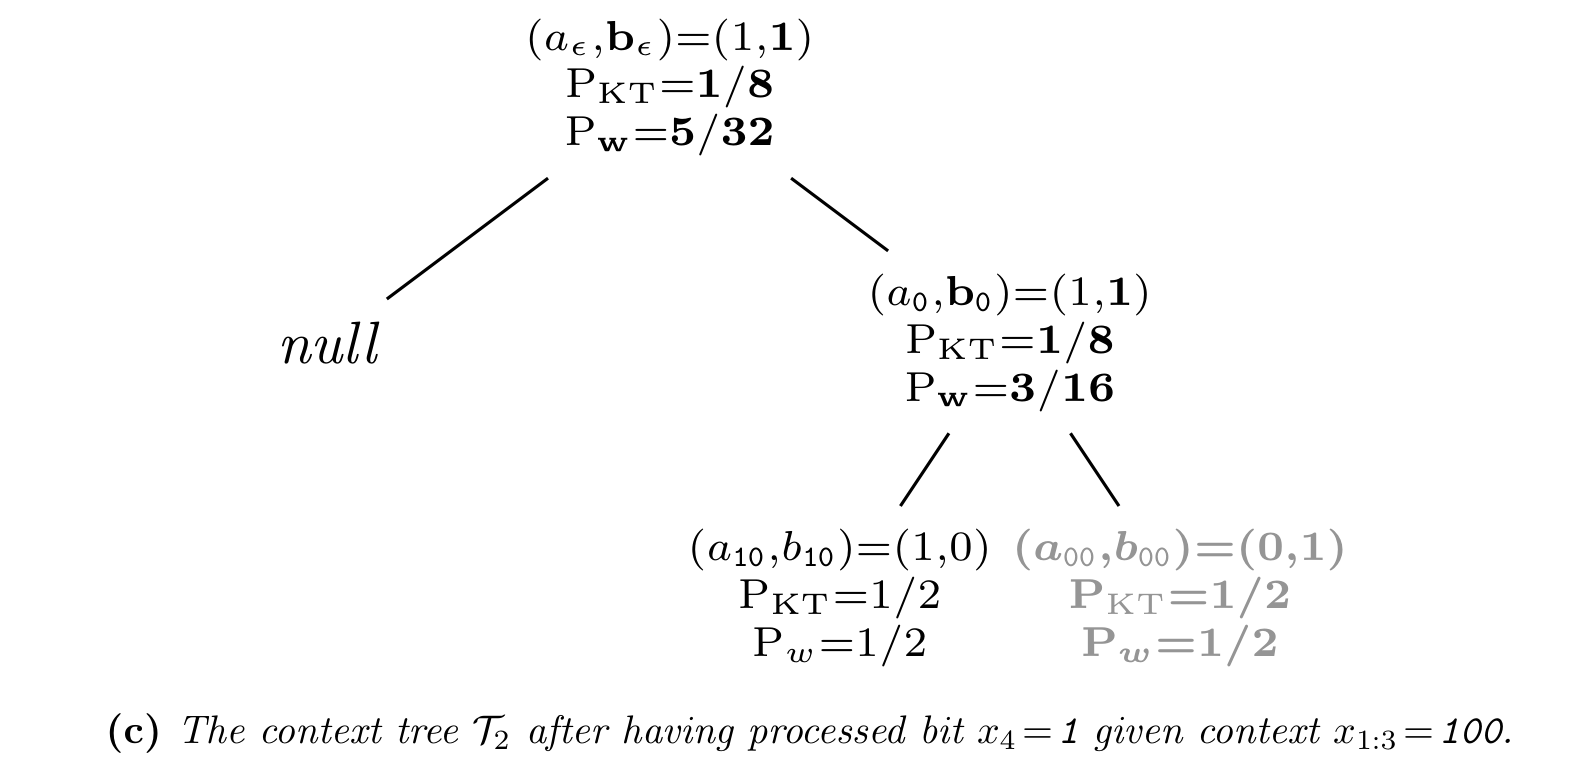
\includegraphics[width=\linewidth]{fig4_13c_online_step2}
\end{column}
\end{columns}
\vspace{0.2cm}
Only the nodes actually visited (black) get allocated; everything else stays \texttt{null}
and contributes exactly $\Pw=1$ — identical results to the fully pre-allocated tree of
Figure 4.11, at a fraction of the memory.

\framebreak

\textbf{3. Reverting changes after prediction.} Algorithm 4.5 needs
$\mathrm{P}_D^{\mathrm{CTW}}(1\,|\,x_{1:t})$, which requires \emph{tentatively} updating the
tree as if $x_{t+1}=\mathtt1$, reading off the new root value, and then undoing that update
before the real next bit arrives. Rather than copying the whole tree, Algorithm 4.7 simply
runs Algorithm 4.6 in reverse: decrement $a_s$ or $b_s$, and invert the KT-probability update
$$
\theta \leftarrow \frac{(a+b+1)}{b+\tfrac12}\,\theta \quad\text{(if $x=1$; symmetric if $x=0$)}
$$
walking down and back up the same path — an $O(D)$-time, $O(1)$-extra-space alternative to
duplicating the tree.
\end{frame}

% ============================================================
\section{4.6 Exercises}
\begin{frame}{Exercises}
\begin{enumerate}
\item [C32m] Prove Lemma 4.1.5 (the lower bound on $\PKT(a,b)$).
\item [C10] Find an explicit closed form for $\PKT(n,n)$.
\item [C10] Construct a countably infinite suffix set that is proper and complete.
\item [C15] Prove that the CTW update (4.5.2) runs in $O(D)$ time.
\item [C15] Repeat the redundancy calculation of Example 4.4.1 for the uneven mixture
$\hat\mu_{w,\alpha}=\alpha\hat\mu_1+(1-\alpha)\hat\mu_2$, and for a general mixture
$\hat\mu_{w,\boldsymbol\theta}=\sum_i\theta_i\hat\mu_i$ with $\theta_i\ge0,\sum_i\theta_i=1$.
\item [C30i] Implement the CTW algorithm and feed it ``random'' bits that \emph{you}
generate by hand. You may find CTW predicts your next bit correctly more than $60\%$ of the
time — humans struggle to act truly randomly!
\item [C35] Derive a multi-alphabet version of CTW (hint: see [PS99]).
\item [C32] Suppose a fixed context compressor can reduce the context length by at least
half. How does this affect CTW's redundancy? Implement this compressed-context version of
CTW and compare it to the original.
\end{enumerate}
\end{frame}

% ============================================================
\section{4.7 History and References}
\begin{frame}[allowframebreaks]{History and References}
\begin{itemize}
\item CTW was first briefly introduced in \textbf{[WST93]}, with an upper bound on the
redundancy. The full explanation and expanded bounds appear in \textbf{[WST95]} — the paper
most often cited as ``the original CTW paper.'' A concise overview by the original authors
is given in \textbf{[WST97]}.
\item The \textbf{KT estimator} itself was originally introduced in \textbf{[KT81]}, as an
efficient, asymptotically-optimal-redundancy estimator for memoryless sources.
\textbf{[SSH12]} discusses a \emph{windowed} version of KT for non-stationary environments
within CTW.
\item \textbf{Multi-alphabet extensions:} \textbf{[TSW93a, TSW93b]} extend CTW to arbitrary
(non-binary) alphabets; one practical approach is to binarize the alphabet
($\mathcal A\hookrightarrow\mathbb B^k$ for $k=\lceil\log_2|\mathcal A|\rceil$)
\textbf{[VH18]}. The \emph{Sparse Adaptive Dirichlet} (SAD) estimator
\textbf{[Hut13a, VH12]} is a near-optimal alternative for large alphabets, later extended to
K-distinct reservoir sampling in \textbf{[Bel15]}.
\item A downside of the original CTW is that the depth $D$ must be fixed in advance;
\textbf{[Wil98]} removes this restriction (at increased computational cost). With $D$
infinite or growing logarithmically in $n$, CTW is asymptotically optimal even on piecewise
stationary sources \textbf{[VCH18]}.
\item Not all sources fit the binary-suffix-tree structure CTW assumes; \textbf{[WST96]}
introduces four new model classes with corresponding weighting algorithms. See
\textbf{[Ris83, RST96]} for more on prediction suffix trees.
\item \textbf{Beyond prediction:} CTW has been applied to active agents via
action-conditional prediction suffix trees \textbf{[VNHS10]} (see Chapter 12). More
recently, \textbf{[MW17]} extends CTW to the interactive/partially-observable case,
yielding \textbf{D2-CTW}, which is less sensitive to aliasing and noise. \textbf{[PS99]}
proposes edge-based (rather than node-based) pruning, considering a larger model class.
\item \textbf{Empirical comparisons:} \textbf{[BEYY04]} compares CTW to other prediction
algorithms in practice, finding it outperforms Lempel-Ziv \textbf{[ZL78, NYEYM03]} and
Prediction by Partial Match \textbf{[CW84, RST96]}.
\item \textbf{Very recently}, \textbf{[GDR+23, GMGH+24]} trained a Transformer (and LSTMs)
on data sampled from CTW, PTW (Section 5.3), and even Solomonoff's distribution. The trained
Transformer nearly perfectly mimics CTW and PTW \emph{in-context} — remarkable, since CTW
and PTW are Bayes-optimal learners of variable-order Markov / piecewise-i.i.d.\ processes
respectively, meaning the Transformer learned to approximate a Bayes-optimal learner purely
from examples, with no further weight updates at test time.
\item \textbf{Looking ahead (Chapter 5):} further variations include adaptive CTW for
non-stationary sources \textbf{[OHSS12]}, Partition Tree Weighting (PTW) for piecewise
stationary sources \textbf{[VWBG13]}, and Context Tree Switching (CTS) \textbf{[VNHB12]}.
\end{itemize}
\end{frame}

% ============================================================
\begin{frame}{Summary}
\begin{itemize}
\item The \textbf{KT estimator} predicts i.i.d.\ Bernoulli sequences with strong,
uniformly-bounded redundancy $O(\log n)$, but cannot exploit any temporal structure.
\item \textbf{$k$-Markov} models add fixed-length context, but the right $k$ is unknown and
costly to over- or under-estimate.
\item \textbf{Prediction Suffix Trees (PSTs)} generalize to \emph{variable}-length context
via suffix sets $\mathcal S$, with a natural \emph{model cost} $\Gamma_D(\mathcal S)$
measuring simplicity.
\item \textbf{Context Tree Weighting} performs an exact Bayesian mixture over \emph{every}
suffix set in $\mathcal C_D$ (up to $2^{2^D}$ of them!) using weights
$w_{\mathcal S}=2^{-\Gamma_D(\mathcal S)}$, updatable in only $O(D)$ time per bit — a genuine
double-exponential speedup over the naive approach.
\item CTW achieves redundancy matching the \textbf{Rissanen lower bound}: it is
asymptotically as good as knowing the true model class member in advance.
\item CTW is not just theory: it is practical, fast, numerically stabilizable (log-domain),
memory-efficient (lazy tree growth), and empirically competitive with state-of-the-art
compressors.
\end{itemize}
\end{frame}

\end{document}
